%%%%%%%%%%%%%%%%%%%%%%%%%%%%%%%%%%%%%%%%%%%%%%%%%%%%%%%%%%%
% --------------------------------------------------------
% Rho
% LaTeX Template
% Version 2.1.0 (14/08/2024)
%
% Authors: 
% Guillermo Jimenez (memo.notess1@gmail.com)
% Eduardo Gracidas (eduardo.gracidas29@gmail.com)
% 
% License:
% Creative Commons CC BY 4.0
% --------------------------------------------------------
%%%%%%%%%%%%%%%%%%%%%%%%%%%%%%%%%%%%%%%%%%%%%%%%%%%%%%%%%%%

\documentclass[9pt,a4paper,twoside]{rho-class/rho}
\usepackage[english]{babel}
\usepackage{graphicx}

%% Spanish babel recomendation
% \usepackage[spanish,es-nodecimaldot,es-noindentfirst]{babel}

\setbool{rho-abstract}{true} % Set false to hide the abstract
\setbool{corres-info}{true} % Set false to hide the corresponding author section

%----------------------------------------------------------
% TITLE
%----------------------------------------------------------

\journalname{Garage Science Ltd}
\title{Investigating the concept of divergent association in large language models}

%----------------------------------------------------------
% AUTHORS AND AFFILIATIONS
%----------------------------------------------------------

\author[1,$\dagger$]{Johnny Kelsey}
%\author[2]{Author Two}
%\author[3,$\dagger$]{Author Three}

%----------------------------------------------------------

%\affil[1]{Affiliation of author one}
%\affil[2]{Affiliation of author two}
%\affil[3]{Affiliation of author three}
%\affil[$\dagger$]{These authors contributed equally to this work}

%----------------------------------------------------------
% DATES
%----------------------------------------------------------

\dates{This manuscript was compiled on August 22, 2024}

%----------------------------------------------------------
% FOOTER INFORMATION
%----------------------------------------------------------

\leadauthor{Kelsey, J.}
\footinfo{Creative Commons CC BY 4.0}
\smalltitle{\LaTeX\ Template}
\institution{College name}
\theday{May 21, 2024} %\today

%----------------------------------------------------------
% ARTICLE INFORMATION
%----------------------------------------------------------

\corres{Johnny Kelsey}
\email{johnny.k.kelsey@gmail.com.}
%\doi{\url{https://www.doi.org/exampledoi/XXXXXXXXXX}}

%\received{March 20, 2024}
%\revised{April 16, 2024}
%\accepted{April 20, 2024}
%\published{May 21, 2024}

\license{Rho LaTeX Class \ccLogo\ This document is licensed under Creative Commons CC BY 4.0.}

%----------------------------------------------------------
% ABSTRACT
%----------------------------------------------------------

\begin{abstract}
    Welcome to rho ($\rho$) \LaTeX\ class for making academic articles and lab reports. In this example template, we will guide you through the process of using and customizing the document to your needs. For more information of this class check out the appendix section. There, you will find codes that define key aspects of the template, allowing you to explore and modify them. If you do not need the abstract set \textit{false} to rho-abstract. It is worth to mention that this template is inspired by an earlier work, the \href{https://es.overleaf.com/latex/templates/tau-class-lab-report-template/chhshmhxstsq}{tau} \LaTeX\ class, designed with academic intentions.
\end{abstract}

%----------------------------------------------------------

\keywords{keyword 1, keyword 2, keyword 3, keyword 4, keyword 5}

%----------------------------------------------------------

\begin{document}
	
    \maketitle
    \thispagestyle{firststyle}
    % \tableofcontents
    \linenumbers

%----------------------------------------------------------

\section{Introduction}

    \rhostart{T}his document is an analysis of the concept of divergent association in large language models (LLMs). It was primarily inspired by the paper "Naming unrelated words predicts creativity"  by Olson and Nahas et al \cite{Olson_2021}. 

The basis concept behind the study is the idea that creative people are able to generate more divergent ideas, and suggest that naming unrelated words and then measuring the semantic distance between them could serve as an objective measure of divergent thinking. The authors tested this hypothesis by devising a test which consisted of participants naming 10 words that are as \emph{different} from each other as possible. The experiment consisted of 8,914 participants, a reasonably large sample size. 

The idea of distance used in this task - words which are as different as possible - can perhaps be grasped intuitively; for instance, the semantic distance between 'cat' and 'dog' would intuitively seem less than the distance between 'cat' and 'cathedral'. We also have computational methods which would provide a more concrete, empirical sense of semantic distance between any two given words. 

The study introduced a new measure of divergent thinking called the Divergent Association Task (DAT). This task asks participants to generate 10 nouns that are as different from each other as possible in all meanings and uses of the words. They then evaluated the results of this task by computing the semantic distance using GloVe \cite{Pennington_2014} \footnote{GloVe is an unsupervised learning algorithm for generating word embeddings by aggregating global word-word co-occurrence matrices from a corpus. A trained GloVe model can be used to encode words into numerical vectors, enabling applications like text classification, sentiment analysis, word analogies, and more.}.  GloVe has also been used in the literature to assess word score tasks used to rank divergent thinking which has previously been used to score the Alternative Uses Task (see Beaty et al  \cite{beaty2021automating}, Dumas et al \cite{dumas2021measuring}). They used a freely available model that was pretrained on the Common Crawl corpus, which contains the text of billions of web pages \cite{Pennington_2014}.

This suggests using the same Divergent Association Task on a number of LLMs, in order to see which can generate divergent word lists, and what the performance of each of the LLMs is at this task in comparison with each other. Can we use DAT to quantify some idea of divergence between the language generating capabilities of LLMs? Will there be a noticeable difference between the "creative" capabilities of large language models? How does the \texttt{temperature} metaparameter affect the divergence of the models? 

\section{Applying LLMs to the divergent words task}

\rhostart{T}he DAT task, as can be found in the original paper \cite{naming-unrelated-words}, is stated below:

\nolinenumbers
\begin{lstlisting}[language=TeX, caption=Original task instructions.]
Instructions
Please write 10 words that are as different from each other as possible, in all meanings and uses
of the words.
Rules
1. Only single words.
2. Only nouns (e.g., things, objects, concepts).
3. No proper nouns (e.g., no specific people or places).
4. No specialised vocabulary (e.g., no technical terms).
5. Think of the words on your own (e.g., do not just look at objects in your surroundings).
6. You will have 4 minutes to complete this task.
\end{lstlisting}
\linenumbers
We will base our prompts to the LLM on this; however, after a brief inspection, we can see that some of these are unnecessary. Instruction 5 might, one day, be useful for multimodal neural networks, but we are not there yet! Similarly, Instruction 6 - humans may need the introversion afforded by four minutes, but an LLM will take seconds to produce text.  

A suggested plain-text prompt would be the following:
\nolinenumbers
\label{humanprompt}
\begin{lstlisting}[language=TeX, caption=Original task instructions.]


I am trying to research how LLMs can be used to generate linguistic diversity. To do this, I need you to generate a list of 10 words.

Here are the instructions:

Please write 10 words that are as different from each other as possible, in all meanings and uses of the words.
Rules
1. Only single words.
2. Only nouns (e.g., things, objects, concepts).
3. No proper nouns (e.g., no specific people or places).
4. No specialised vocabulary (e.g., no technical terms).
5. Just give me the list of words, numbered. 

Please note, I only require a list of 10 words.
\end{lstlisting}
\linenumbers
Note that this prompt was arrived at after some initial experimentation. The LLM was initially rather verbose, so needed to be reminded that we just required a numbered list of 10 words, without any definition of the words, or further expansion - hence that apparent redundancy of \emph{"I only require a list of 10 words"}. 

A relatively quick way to perform this initial experiment would be to decide on a number of LLMs, use the given prompt to apply the DAT test, then assess the divergence of the output words.  

\begin{table*}[pb]
            \RaggedRight
            \caption{LLMs used in DAT test.}
            \label{llmtable}
                \begin{tabular}{lllp{12.2cm}}
                    \toprule
                    \textbf{Name} & \textbf{Build} & \textbf{Size (GB) }  \\ 
                    \midrule
                    Phi-3 & \texttt{lmstudio-community/Phi-3.1-mini-4k-instruct-GGUF/Phi-3.1-mini-4k-instruct-Q4\_K\_M.gguf} & $2.39$ \\
                    Llama-3 & \texttt{lmstudio-community/Meta-Llama-3-8B-Instruct-GGUF/Meta-Llama-3-8B-Instruct-Q4\_K\_M.gguf} & $4.92$ \\
                    Mistral & \texttt{TheBloke/Mistral-7B-Instruct-v0.2-GGUF/mistral-7b-instruct-v0.2.Q4\_K\_S.gguf} & $4.14$ \\
                    Gemma & \texttt{lmstudio-ai/gemma-2b-it-GGUF/gemma-2b-it-q8\_0.gguf} & $2.67$ \\
                    Qwen & \texttt{Qwen/Qwen1.5-7B-Chat-GGUF/qwen1\_5-7b-chat-q5\_k\_m.gguf} & $5.53$ \\
                    \bottomrule
                \end{tabular}
            \tabletext{Note: All LLMs obtained from \texttt{LMStudio}.}
        \end{table*}

\subsection{Divergent association protocol}

The LLMs used are given in \ref{llmtable}; these seemed like a not unreasonable sample of recent language models, which were also capable of running on a single GPU. This method was preferred for reasons of reproducibility, since the models could be reloaded and prompted for responses again under controlled conditions. 

As a quick way of assessing the DAT, we used much the same protocol as the original paper, replacing LLMs with people as our experimental subjects. The models were run twice, once with a default temperature ($0.8$ in \texttt{LMStudio}) and once with the temperature set to the maximum value of $1.0$.  

We adopted the same method to quantify the distance as given in Olson et al's paper \cite{Olson_2021}. They computed the semantic distance using the GloVe embeddings \cite{Pennington_2014}.  This appears to be well-established in the cognitive science literature for this kind of task, as, Olson et al note, it had previously been used to score a similar series of experiments \cite{beaty2021automating} \cite{dumas2021measuring}. We use the 100-dimension GloVe embedding, which was pretrained on the Common Crawl corpus, consisting of several billion web pages.  

Using the prompt given above, we asked the models to generate 10 unique words. The distances between them was assessed using a standard text metric, cosine distance, an implementation of which can be found in the \texttt{SciPy}  library \footnote{\texttt{scipy.spatial.distance.cosine}}. This is given by:

\begin{equation} \label{ec:cosine_distance}
1 - \frac{u \cdot v}{\left|\left|u\right|\right|_{2} \left|\left|v\right|\right|_{2}} \nonumber
\end{equation}
The cosine distance returned is in the interval $[0,1]$; the larger the returned angle between the two vectors, the larger the distance. More precisely:

\begin{itemize}
    \item $0$: orthogonal (independent) vectors
    \item $1$: similar (positive colinear) vectors.
\end{itemize}

A rough-\&-ready way of analysing the divergence of the given word lists would be to simply sum the matrices. A greater sum would indicate a greater divergence.

\section{Divergent association and large language models}

% JKK: let's have a table of the max, mean, std dev
\rhostart{T}he initial results are shown in Table \ref{divergence_res1}. Each of the language models were presented with the prompt, and generated 10 words. The temperature was then raised, from the default of $0.8$ to $1.0$, and the same prompt presented. Observe that the temperature seemed not to make much difference to the divergence of the word lists generated by the models. 

\begin{table}
\caption{LLM cosine distances.}
\label{divergence_res1}
\begin{tabular}{crrrr}
\toprule
\textbf{LLM} & \textbf{Temperature} & \textbf{Sum} & \textbf{Mean} & \textbf{$\sigma$} \\ \hline 
Phi-3 & 0.8 & 73.40 & 0.73 & 0.27 \\
Phi-3 & 1.0 & 71.08 & 0.71 & 0.26 \\
Llama-3 & 0.8 & 79.42 & 0.79 & 0.28 \\
Llama-3 & 1.0 & 79.39 & 0.79 & 0.29 \\
Mistral & 0.8 & 79.51 & 0.79 & 0.29 \\
Mistral & 1.0 & 78.66 & 0.78 & 0.28 \\
Gemma & 0.8 & 61.57 & 0.61 & 0.31 \\
Gemma & 1.0 & 66.95 & 0.66 & 0.31 \\
Qwen & 0.8 & 68.95 & 0.68 & 0.24 \\
Qwen & 1.0 & 78.75 & 0.79 & 0.29 \\ \hline
\end{tabular}
\tabletext{LLM cosine distances: sum, mean and standard deviation.}
\end{table}
A heatmap of the cosine distances yielded by Llama-3 is given in figure \ref{fig:llama3_heatmap}; obviously, the diagonal is zero. 

\begin{figure}
    \centering
    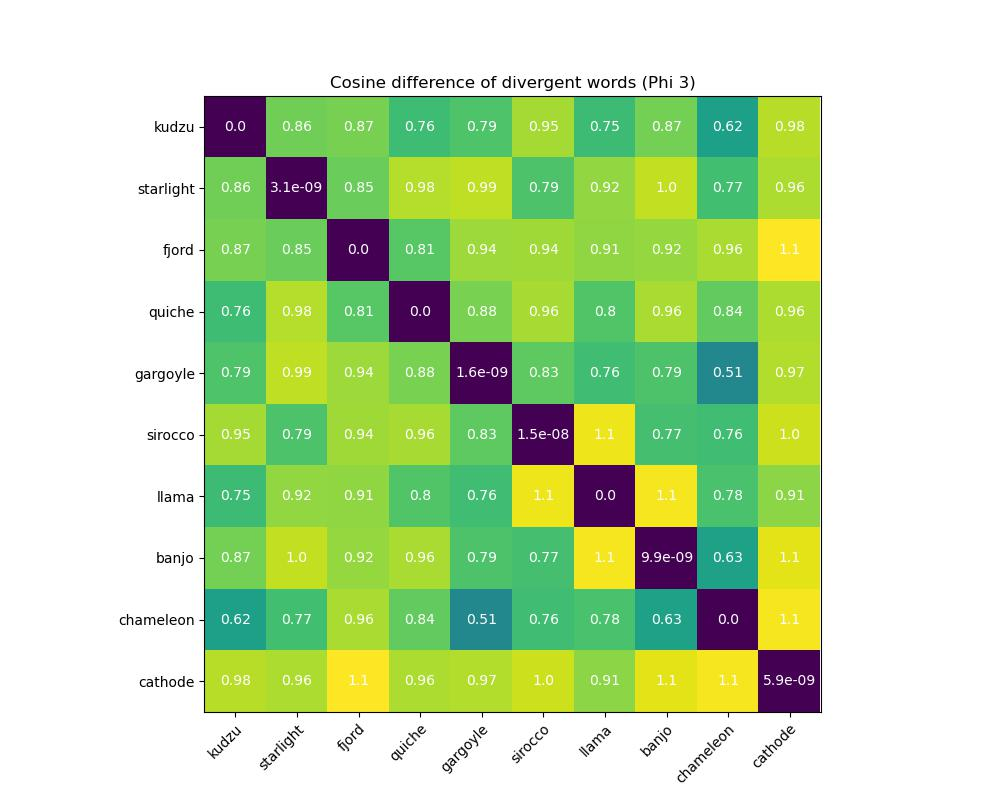
\includegraphics[width=1.3\linewidth]{cos_dist_llama3_3.jpg}
    %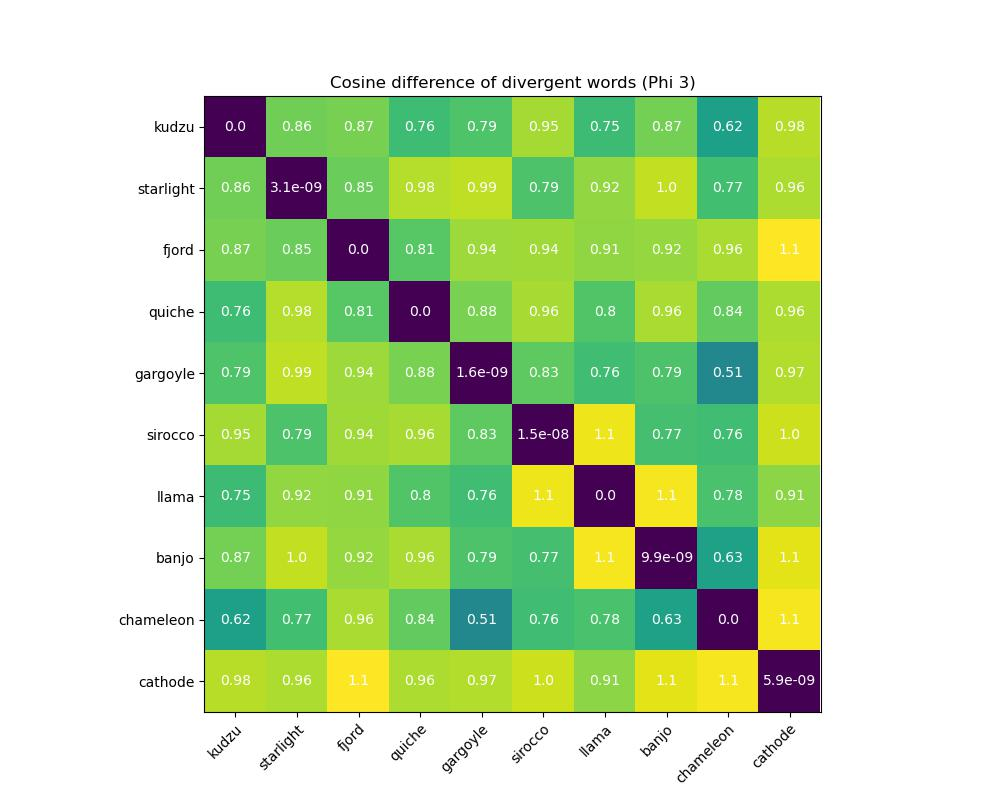
\includegraphics{cos_dist_llama3_3.jpg}
    \caption{Heat map of Llama-3 with temperature 1.0}
    \label{fig:llama3_heatmap}
\end{figure}
Analysing the results, we find that altering the temperature metaparameter makes little difference to the measured divergence of the generated text. It also appears that the size of the model, which varies from $2.39$ to $5.53$ gigabytes, makes little difference to the sum of the distances. 

However, we should ask ourselves: how does this compare to the results, obtained by testing human participants, given in the original paper?

\section{LLM and human divergence}

\rhostart{T}he work by Olson et al \cite{Olson_2021} used human participants in their divergence test. How does our initial experiment with LLMs compare to the human subjects?

Olson and collaborators used the prompt \ref{humanprompt}. They decided to keep only the first seven (valid) words, to, as they put it, "provide redundancy". The DAT score is the transformed average of the semantic distances between these words. This is calculated using cosine distance between all the possible pairs of words, averaged, and then multiplied by 100. 

As they point out, the minimum score (zero) occurs when there is no distance between the words: that is, when all of the words are the same. The theoretical maximum score (200) would occur when the words are as different from each other as possible - bear in mind that they are using a sample of seven words from the participants.  

They found that, in practice, scores commonly range from 65 to 90, and almost never exceed 100. Accordingly, they compare the divergent association task with the grades in an examination, where under 50 could be considered a fail, the average is between 75 and 80, and higher than this could be considered a very high score.

A comparison between human participants and LLMs is made simple by using the original code and embeddings, found at the \texttt{github} repository \footnote{Found at \url{https://github.com/jayolson/divergent-association-task?tab=readme-ov-file}}. The embeddings used were the larger GloVe 300 dimensional vectors, produced using Common Crawl (840 billion tokens, 2.2 million vocabulary, cased, 300 dimensional vectors).  

We can simply run the code over the words produced by our LLMs. We will use all of the ten words in the list, and see what class our models are in from the grading system defined above.

\begin{table}
\caption{LLM cosine distances.}
\label{divergence_res2}
\begin{tabular}{cr}
\toprule
\textbf{LLM}  & \textbf{DAT score} \\ \hline 
Phi 3 & 78.65 \\
Phi 3 & 75.17 \\
Llama 3 & 86.47 \\
Llama 3 & 87.00 \\
Mistral & 83.59 \\
Mistral & 81.20 \\
Gemma & 72.40 \\
Gemma & 76.83 \\
Qwen & 78.75 \\
Qwen & 82.24 \\ \hline
\end{tabular}
\tabletext{LLM DAT results: temperatures $0.8$, $1.0$}
\end{table}

\subsection{Analysis of results}

Table \ref{divergence_res2} shows the results of running the original DAT analysis code over the text which ours LLMs produced. How do our models compare?  

Given that the human participants have an average of 75 6to 80 (depending on demographic breakdown), we can see that the LLMs performed at the high end of the average human score. We used a simple text prompt, varying merely the temperature from the default to the maximum, and used all ten words in the evaluation rather than the first seven. This would provide plenty of scope for further exploration of divergence: for instance, changing the system prompt would likely provide a higher DAT test score.

Olson and their collaborators claim that semantic distance between divergent words correlates with established creativity measures, such as the Alternative Uses Task (see Beaty et al \cite{Beaty_2022}) and the Bridge-the-Associative-Gap Task (Gianotti et al \cite{Gianotti_2001}). As such, we can say that the LLMs we evaluated, with only basic modification of the temperature metaparameter, score at the high end of human divergence association. 

\section{Contact me}

    You can contact me at this email address.\\
    
    \faEnvelope[regular]\hspace{7pt}johnny.k.kelsey@gmail.com \\
%----------------------------------------------------------

\printbibliography

%----------------------------------------------------------

\end{document}